%%%%% Document Setup %%%%%%%%

\documentclass[12pt, onecolumn]{revtex4}    % Font size (12pt) and column number (one or two).

\usepackage[a4paper, left=2.5cm, right=2.5cm,
 top=2.5cm, bottom=2.5cm]{geometry}       % Defines paper size and margin length

\renewcommand{\baselinestretch}{1}     % Defines the line spacing

\usepackage[font=small,
labelfont=bf]{caption}                      % Defines caption font size and caption title bolded

\usepackage{graphics,graphicx,epsfig,ulem}	% Makes sure all graphics works
\usepackage{amsmath} 						% Adds mathematical features for equations

\usepackage{etoolbox}                       % Customise date to preferred format
\makeatletter
\patchcmd{\frontmatter@RRAP@format}{(}{}{}{}
\patchcmd{\frontmatter@RRAP@format}{)}{}{}{}
\renewcommand\Dated@name{}
\makeatother

\usepackage{fancyhdr}


\pagestyle{fancy}                           % Insert header
\renewcommand{\headrulewidth}{0pt}
\lhead{\small Jacky Cao}                        
\rhead{\small The relation between stars and gas in distant galaxies}                

\def\thesection{\arabic{section}}
\def\thesubsection{\alph{subsection}}

\def\bibsection{\section*{References}}        % Position reference section correctly


%%%%% Document %%%%%
\begin{document}                     


\title{The relation between stars and gas in distant galaxies} 
\date{Submitted: \today{}}
\author{Jacky Cao}
\affiliation{\normalfont Level 4 Project, MPhys Theoretical Physics\\ Supervisor: Dr. Mark Swinbank\\ Department of Physics, Durham University}

\begin{abstract}              
 
 Observing any galaxy in the universe will yield the fact that it contains stars and also gas. The dynamics of both can be explored by observing galaxies and collecting spectroscopic data. 
 
Abstract abstract abstract abstract abstract abstract abstract abstract abstract abstract abstract abstract abstract abstract abstract abstract abstract abstract abstract abstract abstract abstract abstract abstract abstract abstract abstract abstract abstract abstract abstract abstract abstract abstract abstract abstract abstract abstract abstract abstract abstract abstract abstract abstract abstract abstract abstract abstract abstract abstract abstract abstract abstract abstract 

\end{abstract}


\maketitle
%\thispagestyle{plain} % produces page number for front page

\tableofcontents
\let\toc@pre\relax
\let\toc@post\relax

\newpage

\section{Introduction} 

Amongst the different types of cosmic structure within our universe, galaxies can be seen as the island powerhouses of industry and activity. Containing countless stars, gas, dust, and dark matter \cite{carroll_astro}, it would be difficult not to express the statement that the motions of these objects must be linked in some form of a galactic relationship. 

By utilising astronomy's most powerful tool, observation, galaxies, their structure and the motions of the objects within them can be studied to a great depth. For example if we took optical measurements of the stellar population, then we could use that information to estimate the potential age of the galaxy. [ref] Or if we wanted to know about the material composition or the distance to that galaxy, we could split the collected light in a spectrograph. [ref]

Gathering and processing this optical and spectroscopic data allows us to build a broad picture of the internal workings of a galaxy. However this picture would not be complete unless we had a general understanding of galaxies themselves. 

\subsection{Galaxy classification}

If we observed a large enough sample of galaxies then we would begin to see that some of them can be grouped together, this categorisation is called the \textit{Hubble Sequence} or the \textit{Hubble Tuning Fork}. With a horizontal handle and two prongs, the sequence itself does not show the evolution of the galaxies, rather it provides a way to view the possible different types of galaxies on one graph. [REF and show an example of the sequence - find some data and plot it? or images of galaxies?] 

We introduced the concept that through optical measurements of the stars 

What do I want to say with this? I want to introduce galaxies, the different types of galaxies, how they form, how they can be confused with other types of structure. 

\subsection{Data} 

Duis eget tellus tortor. Cum sociis natoque penatibus et magnis dis parturient montes, nascetur ridiculus mus. In tellus nulla, sodales eu pulvinar at, accumsan quis magna. Nunc sed lacus diam. Nam enim mauris, imperdiet ut egestas quis, tincidunt at odio. Ut viverra nulla at libero dictum aliquet. Suspendisse lacus lacus, imperdiet nec elit nec, ullamcorper facilisis ex. 

\subsubsection{Hubble Ultra Deep Field} 

\begin{figure}[!h]
\begin{center}
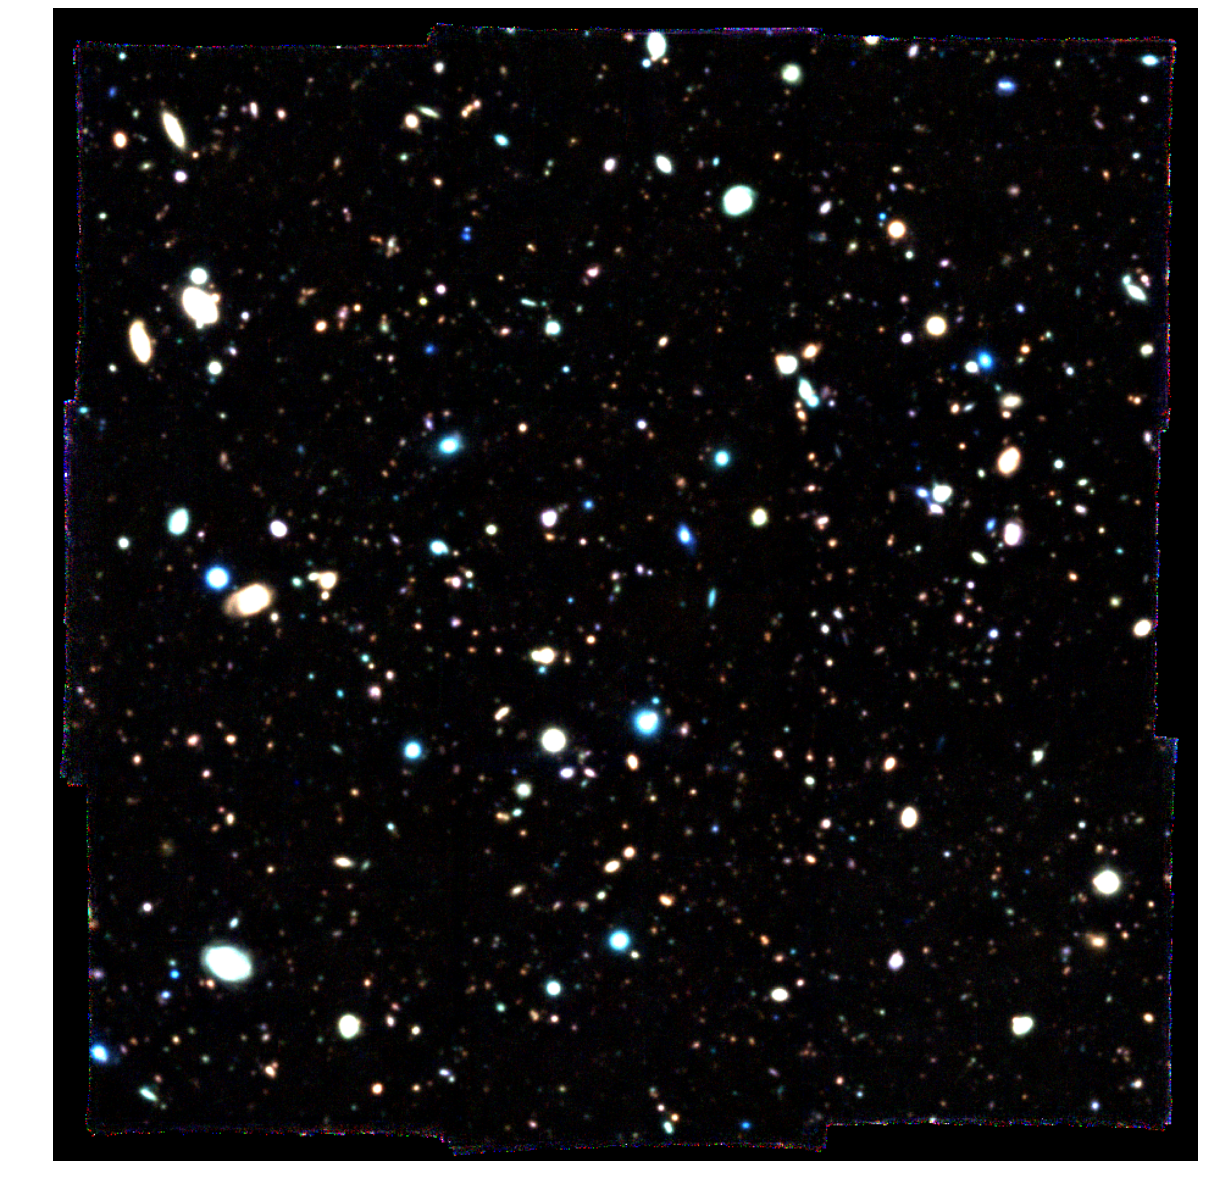
\includegraphics[width=8.5cm]{diagrams/muse_colour_image}
\caption[]{A colour image of the Hubble Ultra Deep Field created using MUSE spectroscopic data. The wavelength range was split into three components, which were then collapsed to create the three colour bands (R, G, B). For every pixel the median value was found from the reduced spectroscopic data. [I NEED TO ADD THE ACTUAL OPTICAL IMAGE FOR A COMPARISON]}
\vspace{-5ex}
\label{fig:muse_colour_image}
\end{center}
\end{figure}

Proin sit amet mauris tincidunt, consectetur nisi ultrices, dapibus elit. Nullam vitae faucibus odio, pharetra ultrices tortor. Class aptent taciti sociosqu ad litora torquent per conubia nostra, per inceptos himenaeos. 

\subsubsection{MUSE} 

To obtain spectroscopic information on the Hubble UDF objects, the Multi-Unit Spectroscopic Explorer or MUSE was employed. This instrument is 

what is MUSE, where it is on the VLT, problems, limitations of MUSE - why it is useful...etc

\section{Analysis} 

\subsection{pPXF} 

Duis eget tellus tortor. Cum sociis natoque penatibus et magnis dis parturient montes, nascetur ridiculus mus. In tellus nulla, sodales eu pulvinar at, accumsan quis magna. Nunc sed lacus diam. Nam enim mauris, imperdiet ut egestas quis, tincidunt at odio. Ut viverra nulla at libero dictum aliquet. Suspendisse lacus lacus, imperdiet nec elit nec, ullamcorper facilisis ex. 

\section{Discussion} 

Duis eget tellus tortor. Cum sociis natoque penatibus et magnis dis parturient montes, nascetur ridiculus mus. In tellus nulla, sodales eu pulvinar at, accumsan quis magna. Nunc sed lacus diam. Nam enim mauris, imperdiet ut egestas quis, tincidunt at odio. Ut viverra nulla at libero dictum aliquet. Suspendisse lacus lacus, imperdiet nec elit nec, ullamcorper facilisis ex. 

\section{Conclusions}
 
Donec finibus, tellus sit amet luctus sodales, lectus ante accumsan ligula, at condimentum lorem justo a sapien. Phasellus vel tortor vitae metus lacinia efficitur ac vel ex. Aenean eget congue leo. Aliquam cursus mauris sit amet arcu dignissim, vel condimentum nisi sodales. 

\begin{acknowledgments}
(OPTIONAL) The author would like to thank...
\end{acknowledgments}

\bibliographystyle{unsrt}
\bibliography{stars_gas_dynamics}

\end{document}